%TEX root = ./overview.tex

\documentclass{standalone}
\usepackage{tikz}
\usepackage{pgfplots}


\pgfplotsset{compat=1.13}

\begin{document}

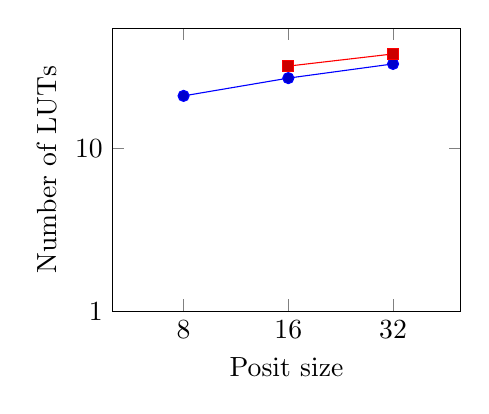
\begin{tikzpicture}
\begin{loglogaxis}[
        log ticks with fixed point,
        width=6cm,
        xmin=5,
        xmax=50,
        ymin=1,
        xlabel={Posit size},
        xtick align=inside,
        xtick={8, 16, 32},
        ylabel={Number of LUTs},
        legend pos=outer north east,
        % x tick label style={font=\normalsize, rotate=45, anchor=east}
        ]
        \addplot coordinates {
        (8,21) (16,27) (32,33)
        };
        \addplot coordinates {
        (16,32) (32,38)
        };
        % \addplot coordinates {
        % (8,21) (16,24) (32,35)
        % };
        % \addplot coordinates {
        % (16,24) (32,33)
        % };
        % \addplot[discard if not both={Expsize}{0}{Operator}{adder}, fill=blue!20] table [x=Size,y=LUT,col sep=comma] {data.txt};
        % \addplot[discard if not both={Expsize}{1}{Operator}{adder}, fill=green!20] table [x=Size,y=LUT,col sep=comma] {data.txt};
        % \addplot[discard if not both={Expsize}{2}{Operator}{adder}, fill=yellow!20] table [x=Size,y=LUT,col sep=comma] {data.txt};
        % \addplot[discard if not both={Expsize}{3}{Operator}{adder}, fill=brown!20] table [x=Size,y=LUT,col sep=comma] {data.txt};
        % \legend{es=0, es=1, es=2, es=3}
      \end{loglogaxis}
\end{tikzpicture}


\end{document}